\documentclass[10pt, onecolumn]{article}

% ---- Geometry & Layout ----
\usepackage[
  a4paper,
  top=2.5cm, bottom=2.5cm,
  left=1.8cm, right=1.8cm,
  columnsep=0.6cm
]{geometry}

% ---- Language & Encoding ----
\usepackage[T1]{fontenc}
\usepackage[utf8]{inputenc}
\usepackage[english]{babel}
\usepackage{csquotes} 

% ---- Fonts ----
\usepackage{lmodern}        % clean vector fonts
\usepackage{microtype}      % better justification / hyphenation

% ---- Mathematics ----
\usepackage{amsmath, amssymb, amsthm}
\usepackage{bm}             % bold math symbols

% ---- Graphics & Colours ----
\usepackage{graphicx}
\usepackage{xcolor}
\usepackage{tikz}           % optional: inline figures
\usepackage{colortbl}

% ---- Tables ----
\usepackage{booktabs}       % professional table rules
\usepackage{tabularx}
\usepackage{multirow}

% ---- Floats ----
\usepackage{float}
\usepackage[font=small, labelfont=bf, labelsep=period]{caption}
\usepackage{subcaption}


% ---- References & Links ----
\usepackage[
  backend=biber,
  maxcitenames=2,    % "et al." dès le 3e auteur en citation
  giveninits=true
]{biblatex}
\addbibresource{Refs.bib}

\usepackage[
  colorlinks=true,
  linkcolor=blue!70!black,
  citecolor=blue!70!black,
  urlcolor=blue!70!black
]{hyperref}

% ---- Miscellaneous ----
\usepackage{lipsum}         % dummy text — remove in real paper
\usepackage{siunitx}        % SI units: \SI{9.81}{\metre\per\second\squared}
\usepackage{enumitem}       % fine-grained list control
\usepackage{indentfirst}


% ============================================================
%  TITLE BLOCK
% ============================================================
\title{%
  \vspace{-1.5em}% pull title closer to top margin
  \Large\bfseries
  A Descriptive and Informative Title:\\
  Subtitle If Needed
}

\author{%
  First Author\textsuperscript{1}\thanks{Corresponding author: \texttt{first@univ.edu}} \and
  Second Author\textsuperscript{1,2} \and
  Third Author\textsuperscript{2}
  \\[0.4em]
  \small\textsuperscript{1}Department of Mechanical Engineering, University Name, City, Country\\
  \small\textsuperscript{2}Institute for Applied Sciences, Another University, City, Country
}

%\date{\small Received: \today \quad|\quad Accepted: \quad|\quad Published:}

% ============================================================
%  DOCUMENT
% ============================================================
\begin{document}

\maketitle
\thispagestyle{empty}  % no page number on title page

% ---- Abstract (single column) ----
    \begin{abstract}
      \noindent

    \end{abstract}
    \vspace{0.5em}
    \noindent\textbf{Keywords:} keyword one; keyword two; keyword three;
    keyword four; keyword five
    \vspace{1em}


% ============================================================
\section{Introduction}
\label{sec:intro}
% ============================================================

%State the motivation and context of the work\cite{example2024}.
%Clearly identify the gap in existing knowledge, then state the objectives
%and contributions of this paper.

%full text

The modeling of a continuum media by a discrete bond network aiming to solve elastic problem dates back to the work of Hrennikoff in the early 1940s \cite{Hrennikoff41}. Although the finite element method eventually replaced bond networks to solve continuum solid mechanics problems, they gained back interest in the field of fracture thanks to their inherent ability to model discontinuities.
The distinct element method was proposed to model granular media by \cite{cundall1979} through the particle to particle interaction of spheres.
The discreate and lattice methods were widely investigated and found to be suitable for the numerical simulation of fracture in brittle materials such as rocks, concrete and ceramics \cite{Schlangen1992, bazant1990, jirasek1994}.

The simplest models consist of axial spring lattices. However, when particles in a lattice only interact through central forces, additional symmetry constraints are enforces by the Cauchy relations. For an isotropic material, the Poisson ratio is fixed to $\nu = \frac{1}{3}$ in 2D and to $\nu = \frac{1}{4}$ in 3D.

To overcome this limitation many scholars enriched this model. Starting with the widely used Born model \cite{Born} which introduces a a non-central two-body interaction, typically an additional tangential spring. The addition of tangential springs may not preserve the rotational invariance and result in an incorrect strain energy \cite{rotationalinvariance}. Alternative approaches were formulated to address this limitation such as beam networks \cite{Schlangen1992, SCHLANGEN19961131, PhysRevE.77.051302, ANDRE2012113} or the combination of axial and angular springs \cite{OSTOJASTARZEWSKI199682, WANG2020102469}. The VCPM and LCM models govern the Poisson ratio through the stiffness of the cell surrounding the struts wich resists volume change \cite{Pan2018LatticeReview, Grassl2006}. The derivation of 4 dimentional axial spring model showed the ability to control the Poisson ration once projected back to 3 dimensions \cite{ZHAO2017881}. Although this method can seem un-natural it maintains the computational simplicity of the axial spring models.

The second problem arising concerns the choice of the bonds stiffness. The microscopic bond properties and the emerging macroscopic ones do not match.
The strain energy equivalence between a network and it's continuum equivalent is commonly employed to choose the microscopic properties. It has been invistaigated in 2D regular lattices \cite{OSTOJASTARZEWSKI199682} and extended to 3D for the 18 neigbors cubic lattice (bond directions [100] and [110]) and for the 14 neigbors cubic lattice (bond directions [100] and [111]) \cite{LADD1997349, Kot2015}. This method has been applied to estimate the emerging Young's modulus of disordered lattices with uniform spring stiffness \cite{Kot2015}. Conversly, it was locally applied to each cell of a 3D arbitrary mesh in order to derive the normal and angular spring stiffnesses required to obtain an isotropic behavior with a set Young's modulus and Poisson ratio \cite{Reck2017LatticeSM}. 


Typical DEM networks use the same material parameters for all bounds which is simpler but means the isotropic behavior relies on the isotropy of the bond's orientations and can only be seen at the macroscopic scale \cite{ANDRE2012113}. On the other hand the energetic parametrisation gives an exact solution such that one unit cell is isotropic.
For beam lattices, the choice of microscopic stiffnesses relies on a lengthy calibration process. The typical calibration process is a trial and error calibration that requires multiple tensile tests until matching the desired behavior \cite{ANDRE2012113}. To speed up this process analytical curves have been fitted to several pre-made numerical tensile tests \cite{NGUYEN2019393}. An other approach is to take the bound's parameters as additional coordinates of the problem and solving it through a proper generalised decomposition\cite{GIRARDOT2021993}.

%\subsection {good lattice criteria}
%\cite{VAIANI2025110442} lists guidline for the optimal distribution of springs in an LSM as : 
%\begin{itemize}
%    \item Intrinsic rigidity of the lattice
%    \item Homogeneity (uniformity in springs lengths) \textcolor{red}{in the case of refined meshes the spring length homogeneity is not respected at all but we must keep in mind that in the articles they establish this rule by assuming the stiffness of spring to be homogenous which we don't}
%    and isotropy (uniformity in springs orientations). For exemple periodic unit cells have a very narrow diversity in spring orientations which makes the crack paths highly mesh dependant as observed by \cite{SCHLANGEN1997319}. Randomness in the nodes placement is often introduced to diminish the mesh's influence (\cite{Kot2015}). 
%    \item Boundary conformity
    
%\end{itemize}

% ============================================================ Energy equivalence ============================================================
\section{Energy equivalence method}

Elate Software : \cite{Gaillac_2016}

    \begin{itemize}
        \item The goal is to match the strain energy of a RVE of the spring network to the strain energy of an equivalent continuous volume with the required behaviour.
        \item To deduce the final system we make the following assumptions :
        \begin{itemize}
            \item Cauchy-Born rule : assumes that the displacements of the nodes follow the macroscopic strain and is linearised around each cell's center.
            \item Major and minor symetries of the homogensied stiffness tensor.
        \end{itemize}
        As shown by \cite{Yin2023} these conditions are met by central symmetric lattices but might not be for a general lattice.
        \item Final analytical expression of the homogenised stiffness tensor through energy equivalence :
        \begin{equation}
C_{\alpha\beta\gamma\delta} = \sum_{ij} \frac{k_{ij}\|\underline{x}_{ij}\|^2}{ V}\, n_{ij,\alpha}\, n_{ij,\beta}\, n_{ij,\gamma}\, n_{ij,\delta}
\label{homogenised tensor}
\end{equation}
\item showing the isotropic stiffness matrix we need to match :
\begin{equation}
C_{\alpha\beta\gamma\delta} = \lambda\, \delta_{\alpha\beta}\delta_{\gamma\delta} + \mu\left(\delta_{\alpha\gamma}\delta_{\beta\delta} + \delta_{\alpha\delta}\delta_{\beta\gamma}\right)
\end{equation}
with the Lamé coefficients :
\begin{equation}
\lambda = \frac{E\nu}{(1+\nu)(1-2\nu)}, \qquad \mu = \frac{E}{2(1+\nu)}
\end{equation}
\item show addition symmetry leading to nu = 0.25
\begin{equation}
\mathbb{C} = \sum_{ij} \underbrace{\frac{k_{ij} \|\underline{x}_{ij}\|^2}{V}}_{\equiv K_{ij}}
\underbrace{
\left(
\begin{array}{cccccc}
n_1^4 & \cellcolor{yellow!40} n_1^2 n_2^2 & n_1^2 n_3^2 & n_1^2 n_2 n_3 & n_1^3 n_3 & n_1^3 n_2 \\
\cellcolor{yellow!40} n_1^2 n_2^2 & n_2^4 & n_2^2 n_3^2 & n_2^3 n_3 & n_1 n_2^2 n_3 & n_1 n_2^3 \\
n_1^2 n_3^2 & n_2^2 n_3^2 & n_3^4 & n_2 n_3^3 & n_1 n_3^3 & n_1 n_2 n_3^2 \\
n_1^2 n_2 n_3 & n_2^3 n_3 & n_2 n_3^3 & n_2^2 n_3^2 & n_1 n_2 n_3^2 & n_1 n_2^2 n_3 \\
n_1^3 n_3 & n_1 n_2^2 n_3 & n_1 n_3^3 & n_1 n_2 n_3^2 & n_1^2 n_3^2 & n_1^2 n_2 n_3 \\
n_1^3 n_2 & n_1 n_2^3 & n_1 n_2 n_3^2 & n_1 n_2^2 n_3 & n_1^2 n_2 n_3 & \cellcolor{yellow!40} n_1^2 n_2^2
\end{array}
\right)
}_{ \mathbb{N}_{ij} \equiv \displaystyle [\underline{n}_{ij}^{\otimes 4}]_{\text{Voigt}},\quad \text{notation}: n_\alpha \equiv n_{ij,\alpha}}
\label{detailed energy match}
\end{equation}

The fourth order tensor $\underline{n}_{ij}^{\otimes 4}$  has the same major and minor symmetries as $\mathbb{C}$ and an additional symmetry due to the commutativity of product. $\mathbb{N}_{ij, \alpha \alpha \beta \beta} = \mathbb{N}_{ij, \alpha \beta \alpha \beta} $
(an example of this additional symmetry is colored in the matrix above).

\item This additional symetry + isotropy --> Cauchy relation (nu = 0.25)
\\This additional symmetry confirms the Cauchy relation in the case of an isotropic $\mathbb{C}$ 
\begin{equation}
\left(
\begin{array}{cccccc}
\lambda + 2\mu & \cellcolor{yellow!40} \lambda & \lambda & 0 & 0 & 0 \\
\cellcolor{yellow!40} \lambda & \lambda + 2\mu & \lambda & 0 & 0 & 0 \\
\lambda & \lambda & \lambda + 2\mu & 0 & 0 & 0 \\
0 & 0 & 0 & \mu & 0 & 0 \\
0 & 0 & 0 & 0 & \mu & 0 \\
0 & 0 & 0 & 0 & 0 & \cellcolor{yellow!40} \mu
\end{array}
\right)
= \sum_{ij} \frac{k_{ij} \|\mathbf{x}_{ij}\|^2}{V}
\left(
\begin{array}{cccccc}
n_1^4 & \cellcolor{yellow!40} n_1^2 n_2^2 & n_1^2 n_3^2 & n_1^2 n_2 n_3 & n_1^3 n_3 & n_1^3 n_2 \\
\cellcolor{yellow!40} n_1^2 n_2^2 & n_2^4 & n_2^2 n_3^2 & n_2^3 n_3 & n_1 n_2^2 n_3 & n_1 n_2^3 \\
n_1^2 n_3^2 & n_2^2 n_3^2 & n_3^4 & n_2 n_3^3 & n_1 n_3^3 & n_1 n_2 n_3^2 \\
n_1^2 n_2 n_3 & n_2^3 n_3 & n_2 n_3^3 & n_2^2 n_3^2 & n_1 n_2 n_3^2 & n_1 n_2^2 n_3 \\
n_1^3 n_3 & n_1 n_2^2 n_3 & n_1 n_3^3 & n_1 n_2 n_3^2 & n_1^2 n_3^2 & n_1^2 n_2 n_3 \\
n_1^3 n_2 & n_1 n_2^3 & n_1 n_2 n_3^2 & n_1 n_2^2 n_3 & n_1^2 n_2 n_3 & \cellcolor{yellow!40} n_1^2 n_2^2
\end{array}
\right)_{ij}
\end{equation}

\item Need a max of 15 different orientations to have a basis. \cite{Reck2017LatticeSM} does this with additional angular springs -> 21 component to for a base and can adapt the poisson.  
    \end{itemize}

    Show the symmetry in this equation that sets the poisson ratio to 0.25 (in 3D)

    Monter qu'on peut mettre la longueur des bonds en évidence et uniquement trvailler avec des orientations -> on résoud le meme systeme pour une cellule plus grande ou plus petite -> avec la proportion sur les longueurs et le volume représentatif.

% ============================================================ undeformed cubic cell ============================================================

\section{Undeformed cubic periodic cells}
    \begin{itemize}
        \item Face centered result
    \begin {figure}[H]
        \centering
        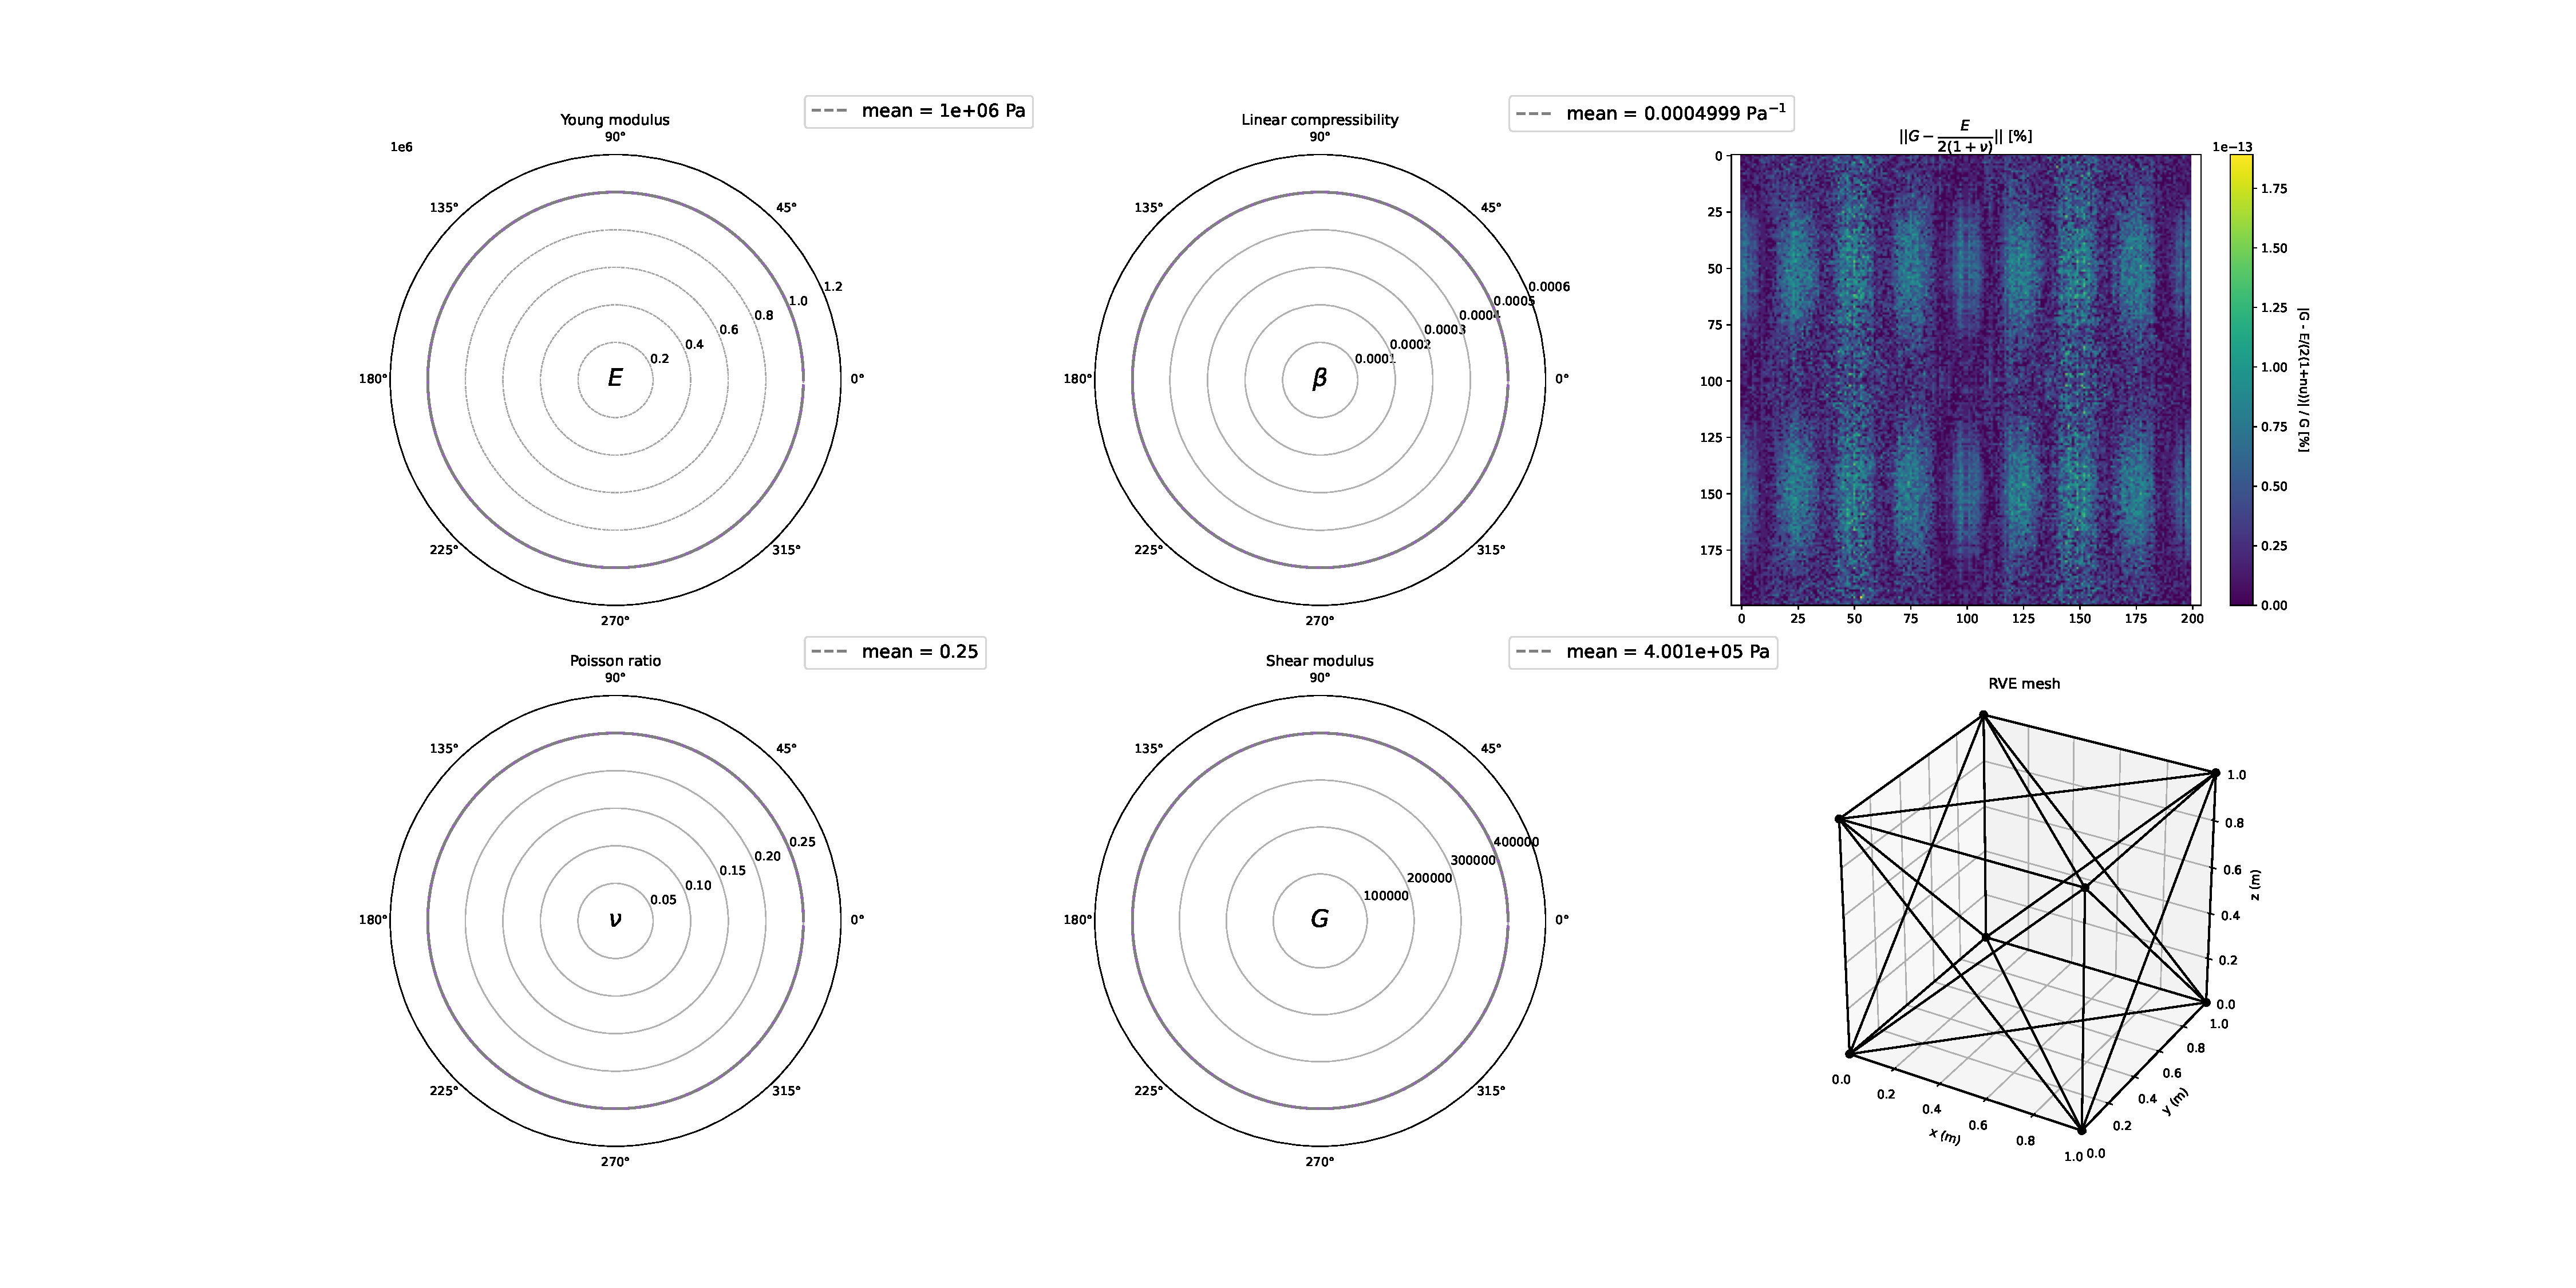
\includegraphics[width=0.8\textwidth]{images/Undeformed_cubic_periodic/face_diagonal_periodic.pdf}
        \caption{}
        \label{fig:FCC homogenisation}
    \end{figure}

        \item Body centered result (that is by the way the smallest amount of bonds we can have in a cubic symetric cell -- demo in annex ??)
        \begin {figure}[H]
            \centering
            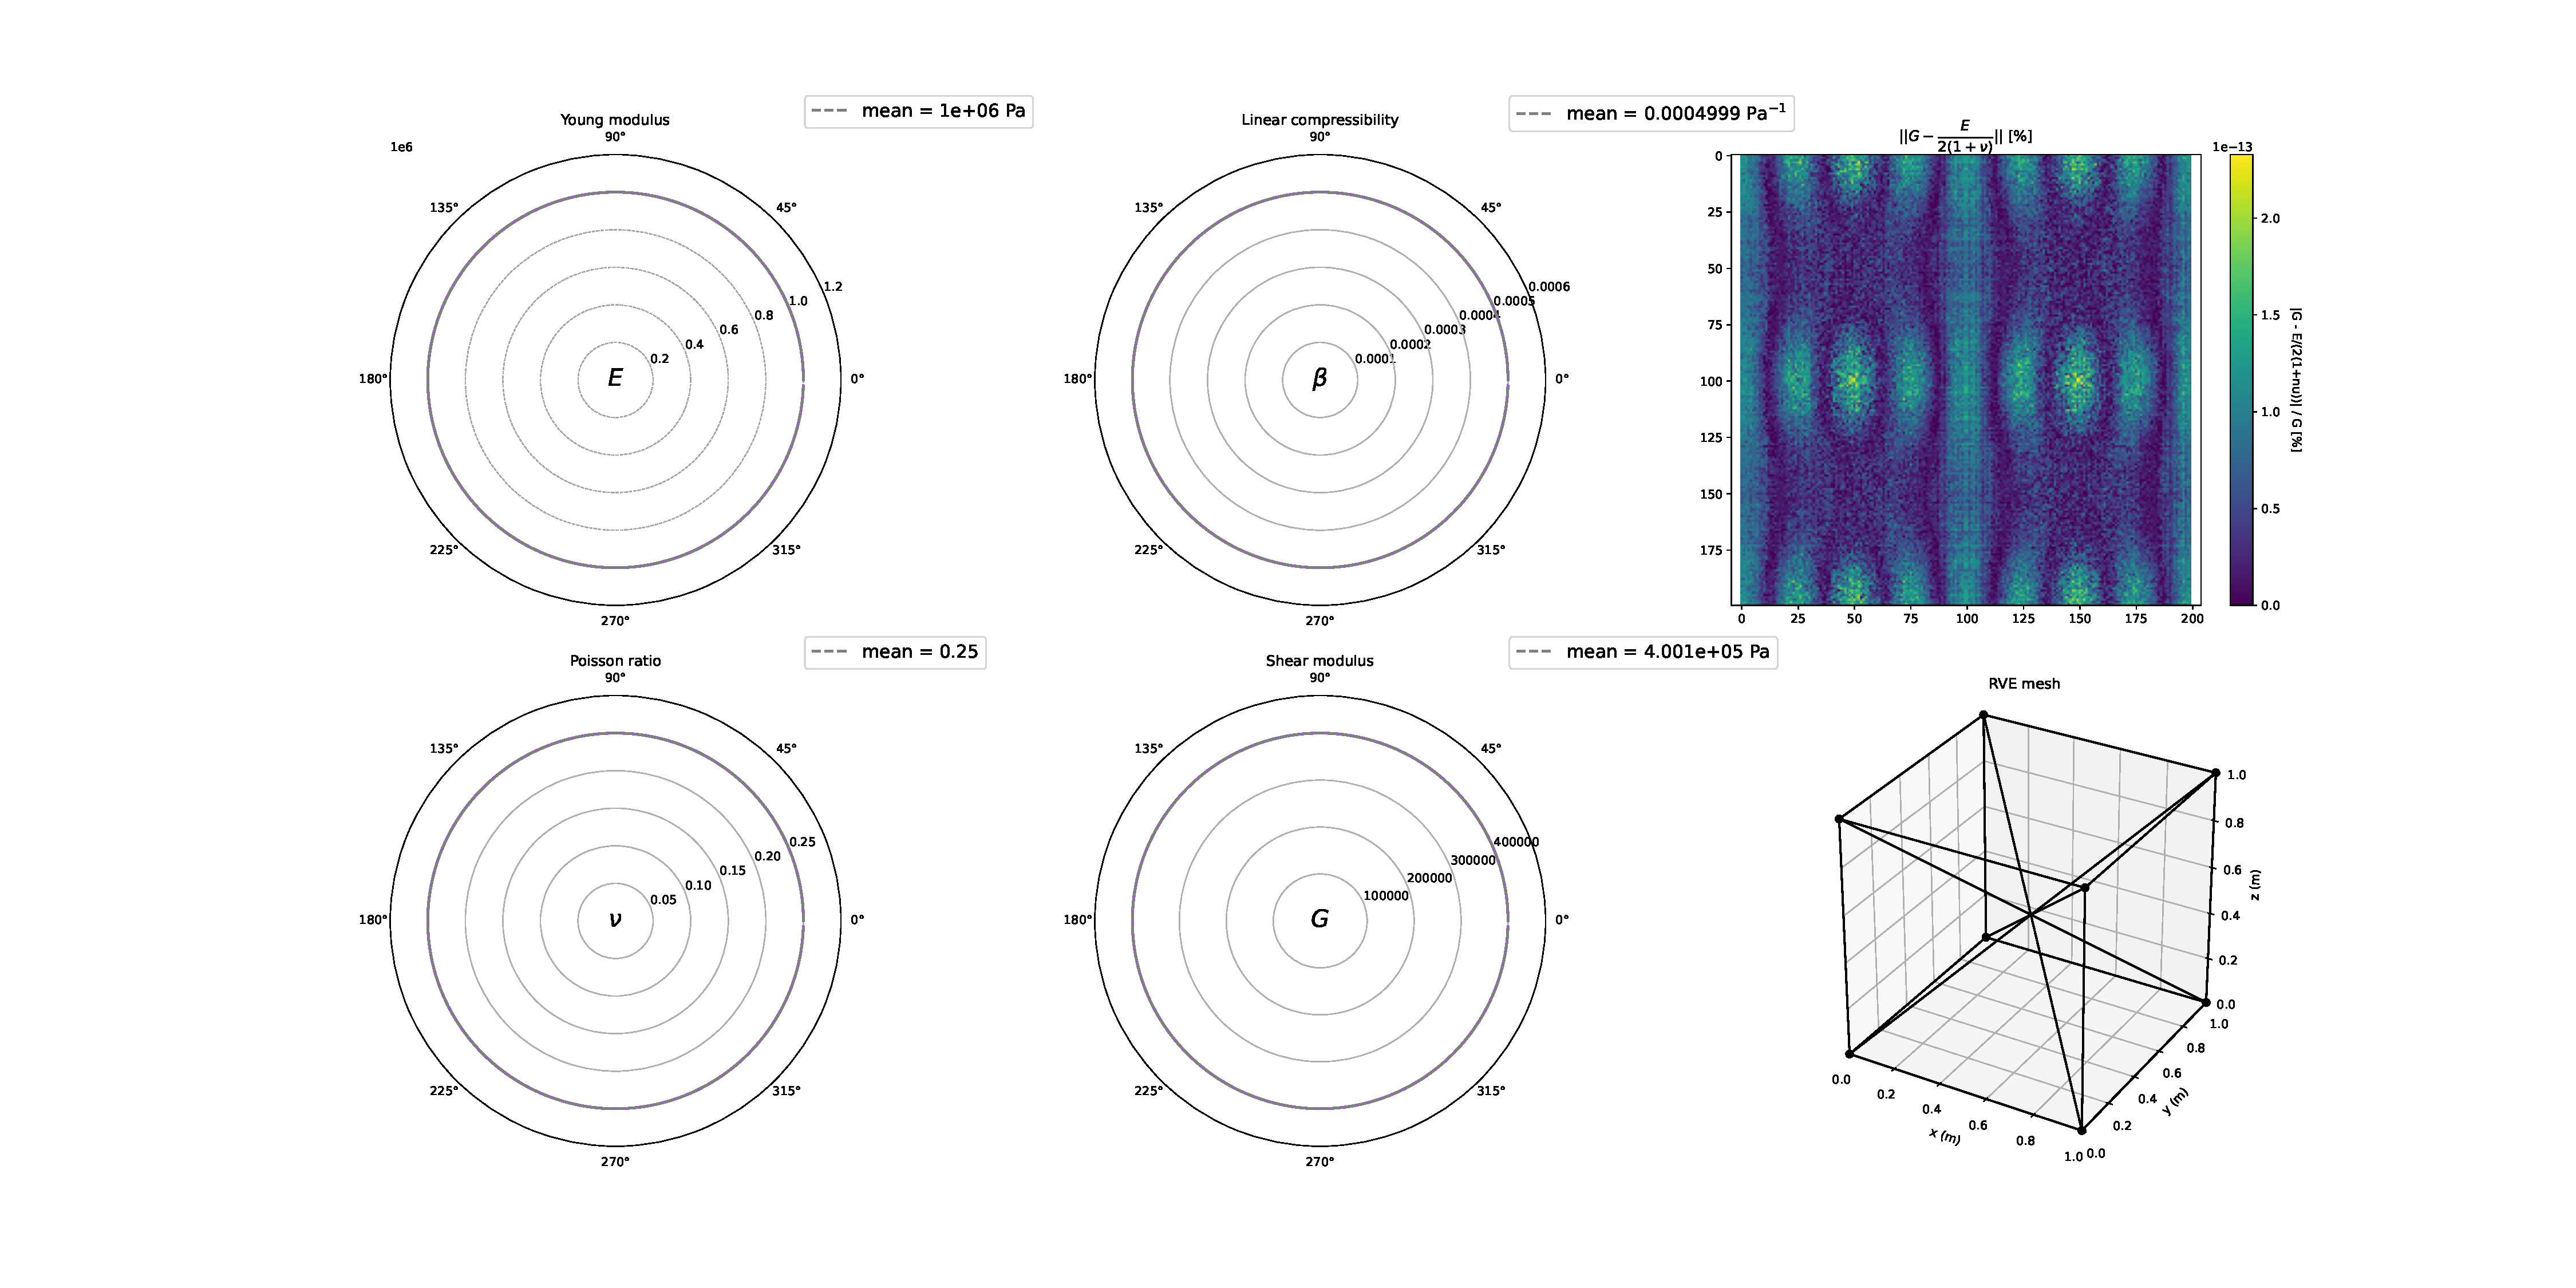
\includegraphics[width=0.8\textwidth]{images/Undeformed_cubic_periodic/cube_diagonal_periodic.pdf}
            \caption{}
            \label{fig:BCC homogenisation}
        \end{figure}
    \end{itemize}

    Give the analytical redults for the BCC / FCC geometries and show that the numerical homogenisation confirms the analytical result

\section{Deformed hex cell}
    1/ justify the number of bonds per cell in order to be able to solve the system
    Show exemples of deformed cells
    \begin{itemize}
        \item parallelepiped -> the rank of the matrix is 12 not 15 but still enough to solve the system by "chance"
        \item \begin {figure}[H]
            \centering
            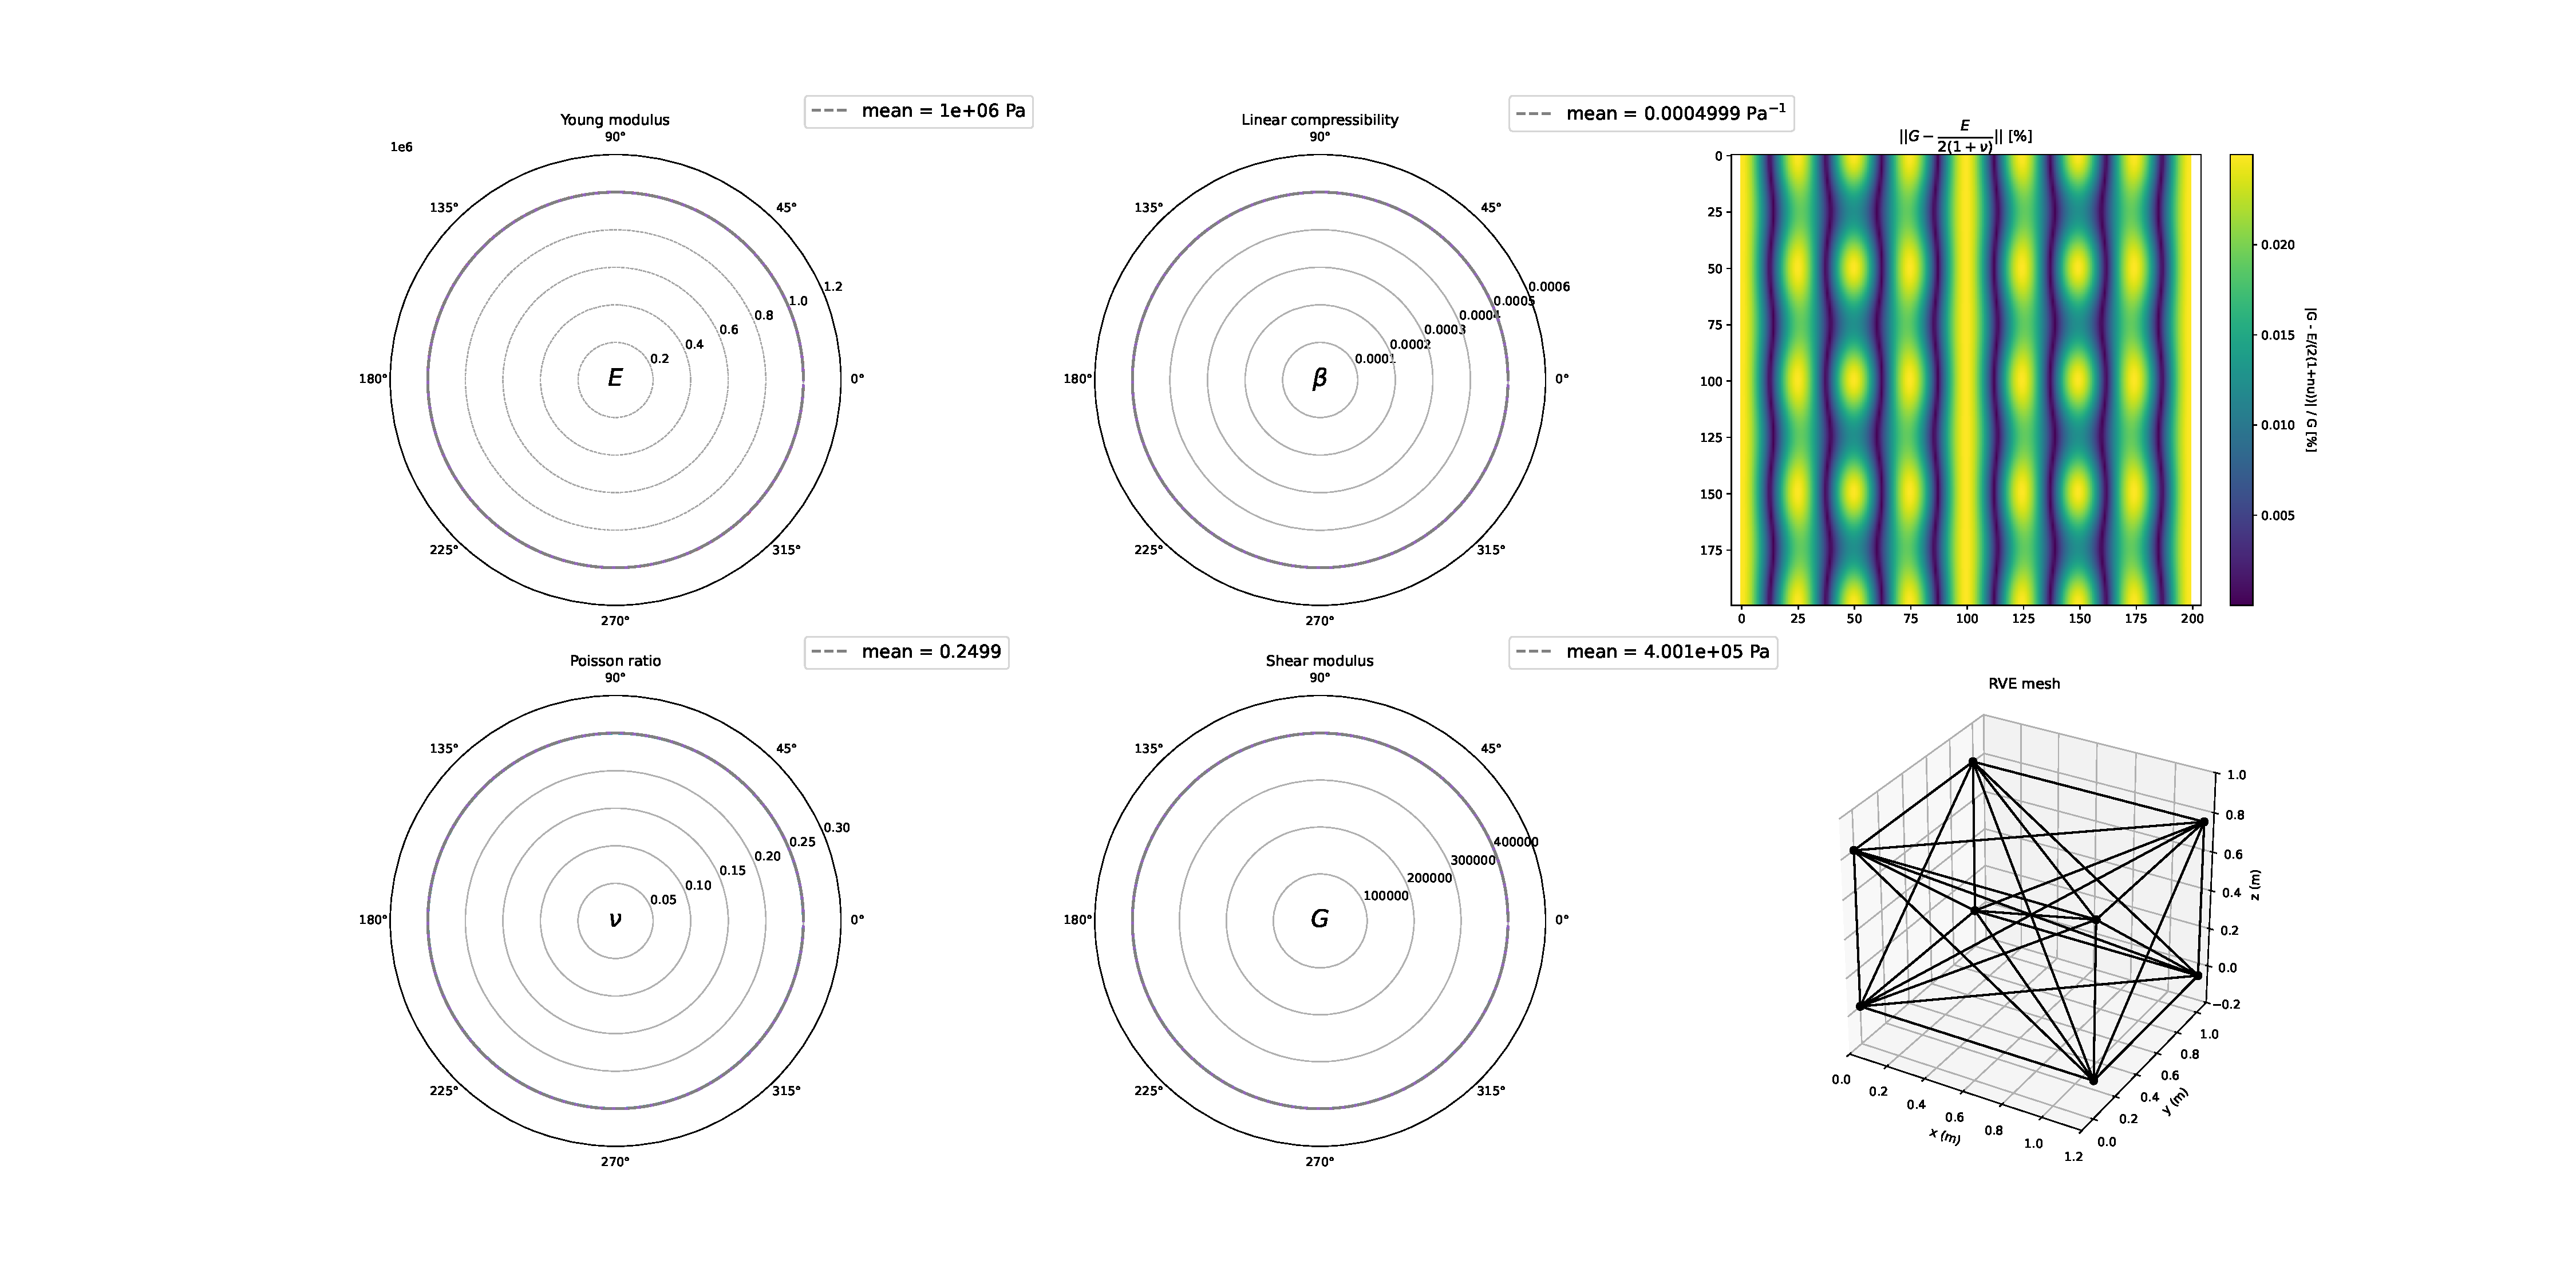
\includegraphics[width=0.8\textwidth]{images/Deformed_hex/parallelepipede_non-periodic.pdf}
            \caption{}
            \label{fig:parallelepiped homogenisation}
        \end{figure}
        \item "corner" -> the rank is 15 -> can be solved
        \item \begin {figure}[H]
            \centering
            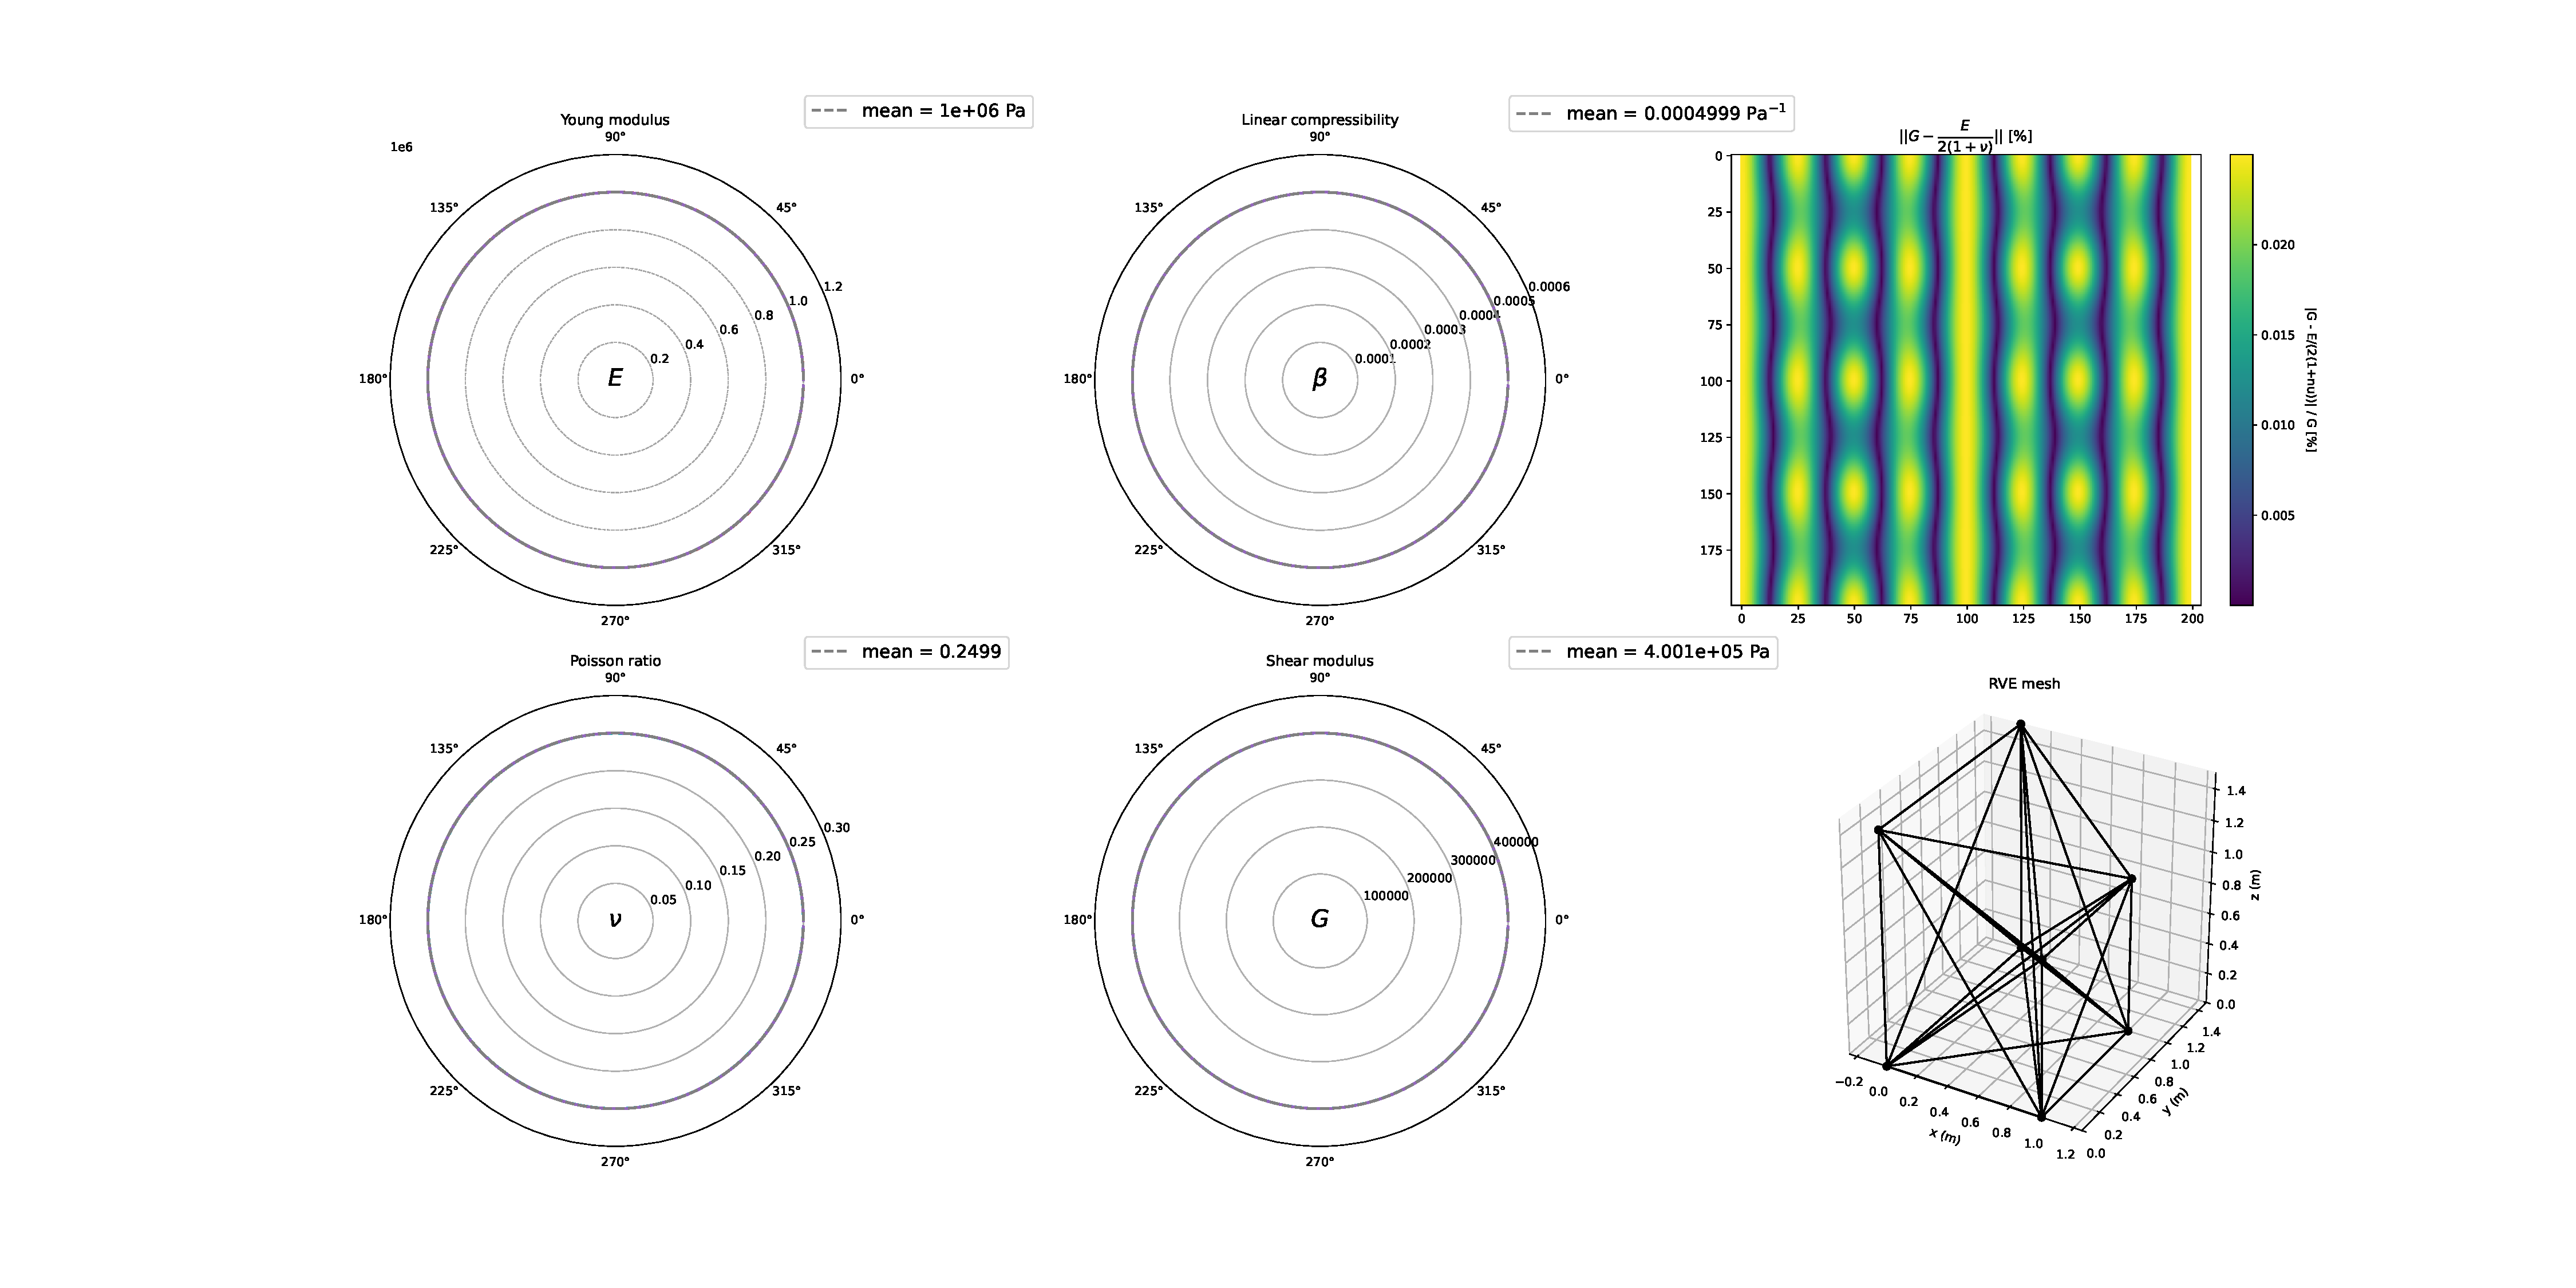
\includegraphics[width=0.8\textwidth]{images/Deformed_hex/angle_non-periodic.pdf}
            \caption{}
            \label{fig:corner homogenisation}
        \end{figure}
        
        \item sheared -> not working, not enough orientations (rank 12)
        \item \begin {figure}[H]
            \centering
            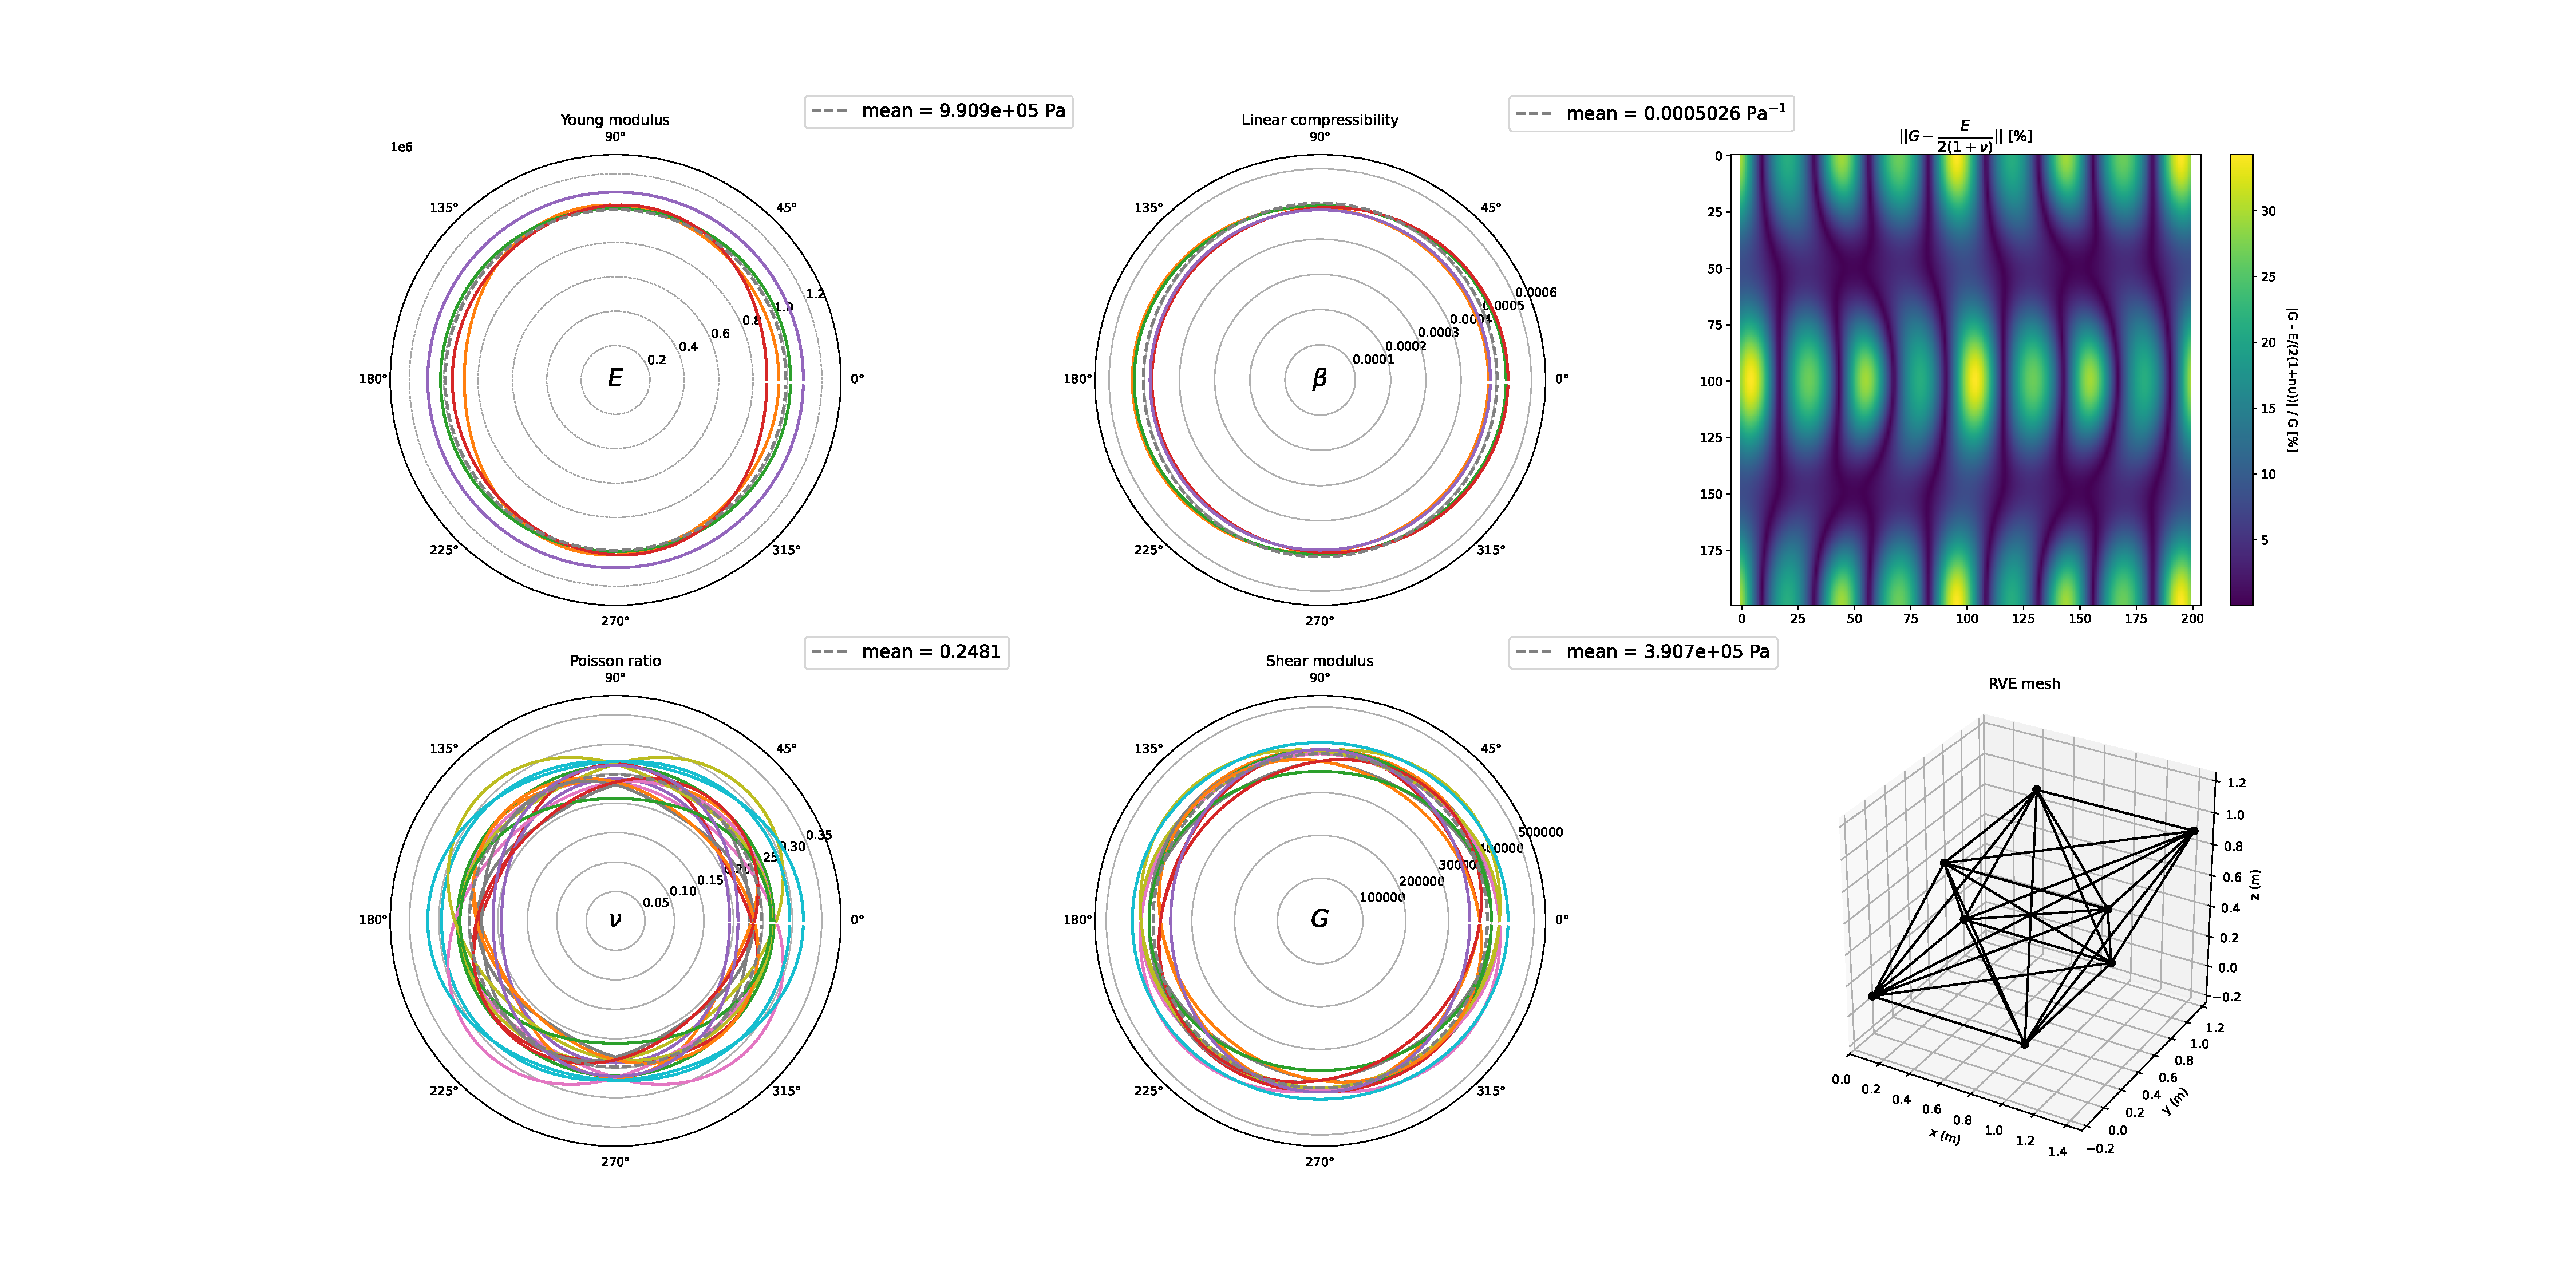
\includegraphics[width=0.8\textwidth]{images/Deformed_hex/shear_non-periodic.pdf}
            \caption{}
            \label{fig:shear homogenisation}
        \end{figure}
    \end{itemize}

    -> takes a lot of time to solve each cell independently
    Show analytical mapping is not possible and no even a function
        not possible analytically due to the degree of the equation and not even a function as we saw that the sheared cell was not solvable
    
% ============================================================ Deformed hexahedral cell ============================================================
\section{Mesh of deformed hex -> need a faster parametrisation}
    \subsection{problems with the cell by cell calibration}

    3/ show the results are not accurate when we add randomness because we are violating the linear displacement hypothesis -> show the high variation in stiffnesses. 
    Calibration each cell independently has multiple problems :
    \begin{itemize}
        \item The calibration is time consuming (requires to solve a 15x15 system for each cell)
        \item There is no guarantee that a solution with all positive stiffnesses exists.
        \item There is no guarantee that a solution exists
        \item for a hex cell to be solvable it needs 15 different orientations. (in our case we use a coordination number of 22 which is very high)
        \item The solution indeed gives a perfectly homogenised stress tensor only if the free nodes follow the cauchy rule. 
        \textcolor{red}{generate the graph that shows the variation in displacement relative to the cauchy Born rule}
    \end{itemize}

    A way to fasten the calibration would be to find a solution that maps the stiffnesses of a reference cell (in the case presented in the "Deformed hex cell" section above the reference cell would be a cubic cell with [100], [110] and [111] bonds)
    Let's consider a reference configuration with a set of bonds orientations $\xi \in R(24 X 3)$, the deformed orientations can be expressed as a linear combination of the reference configuration.
    $n = A \xi$ wit A a 24X24 matrix. When introduced in the energy equivalence equation we get a 4th order polynomial of the components of which cannot be solved analytically. Therefore it comes back once again to solving a numerical system for each cell.  
    \subsection{idea of the equivalen cell parametrisation}
    Instead of solving each cell independently we require isotropy only at the macroscopic scale. Which asks to solve the energy equivalence equation a single time summing the contribution of all the bonds. However this sytem grows fast with the number of bonds and doesn't garantee any homogeneity of the stiffness through the mesh. Therefor we propose an other methodology with the following steps :
    \begin{itemize}
        \item Categorise the bonds depending on their orientation (For that we use Healpix of order 4 -> all categories cover the same section of the sphere)
        \item compute the mean representative bond of each category
        \item solve the energy equivalence on this set of equivalent bonds. We solve the following equation :
        \begin{equation}
    \mathbb{C} \, V_{total} = \sum_{c \in \textit{bond categories}} k_{eq, c} \,
    \underline{n}_{eq, c}^{\otimes 4} = \sum_{ij \in \textit{bonds}} k_{ij} \|\mathbf{x}_{ij}\|^2 \,
    \underline{n}_{ij}^{\otimes 4} \approx \sum_{c \in \textit{bond categories}} \left( \sum_{ij \in \textit{c}} k_{ij} \|\mathbf{x}_{ij}\|^2 \right) \,
    \underline{n}_{eq, c}^{\otimes 4} 
    \label{equivalent cell energy match}
\end{equation}
        -> the stiffness found here is the stiffness that all the bonds from this category must have together.
        \begin{equation}
            k_{eq, c} = \sum_{ij \in \textit{c}} k_{ij} \|\mathbf{x}_{ij}\|^2
            \label{repartition criteria}
        \end{equation}
        \item the equation \eqref{repartition criteria} gives us a rule on the combined stiffness in a given orientation but not on how it should be split between bonds of a same orientation. Although an intuitive choice might be to take the same stiffness for all bonds of the same direction. When refining the mesh that will cause stiffer zones when the bond density is higher. 
        Let's consider the following situation, a mesh is composed of cells with identical bond orientations but different scales. 
        \textcolor{red}{include an exemple image with 2 zones}
        We would like both cells to have the same energy density ie.
        \begin{equation}
            \sum_{ij \in \textit{bond cell 1}} \frac{k_{1,ij} \|\mathbf{x}_{1,ij}\|^2}{V_1} \,\underline{n}_{1,ij}^{\otimes 4} = \sum_{ij \in \textit{bond cell 2}} \frac{k_{2,ij} \|\mathbf{x}_{2,ij}\|^2}{V_2} \,\underline{n}_{2,ij}^{\otimes 4}
        \end{equation}
        as the orientations are the same ($\underline{n}_{1,ij}^{\otimes 4} = \underline{n}_{2,ij}^{\otimes 4} \forall ij$), by identification we must have :
        \begin{equation}
            \frac{k_{1,ij} \|\mathbf{x}_{1,ij}\|^2}{V_1}  = \frac{k_{2,ij} \|\mathbf{x}_{2,ij}\|^2}{V_2}
        \end{equation}

        We can take this term out of the sum in \eqref{repartition criteria}, resulting in :
        \begin{equation}
            k_{ij} = \frac {k_{eq, c} \, V_{cell, ij}}{\|\mathbf{x}_{ij}\|^2 \, \sum_{ij \in c} V_{cell, ij}}   \qquad  \forall ij \in c
            \label{repartition criteria mis en evidence}
        \end{equation}

    \end{itemize}
    \subsection{test of the equivalent cell parametrisation on flexion test case}

         Regular meshing OK
        Change orientaion KO
        Refinement KO
            -> Heterogeneity in the orientation repartion and in the density either work on more local parts of the mesh -> hard to automate)



% ============================================================ Thetrahedral cell ============================================================

\section{Thetrahedrons}
    because a tet cell cannot periodically pave the 3D space it will typically show more diversity in orientations.
     We can therefore assume that all bond categories are represented and each category must have the same combined stiffness.
     \textcolor{red}{add the demo detail with the sum of fabric tensors already producing isotropy}
     + reuse the length² / volume proportion. 




% ============================================================
\section{Discussion}
\label{sec:discussion}
% ============================================================



% ============================================================
\section{Conclusion}
\label{sec:conclusion}
% ============================================================

Summarise the key findings and their implications. Avoid introducing new
material here. Optionally, state perspectives for future work.



% ============================================================
%  ACKNOWLEDGEMENTS
% ============================================================
\section*{Acknowledgements}

The authors thank \ldots{} for \ldots{}
This work was supported by [funding agency] under grant [number].

% ============================================================
%  APPENDIX (optional)
% ============================================================
\appendix
\section{Derivation of Equation}~\eqref{homogenised tensor}
\subsection{Writting the energy of the spring lattice}
The strain energy stored in a unit cell of volume V is
\begin{equation}
W = \sum_{ij \, \in \, bonds} \frac{k_{ij}}{2}\left[(\underline{u}_j - \underline{u}_i)\cdot \underline{n}_{ij}\right]^2
= \sum_{ij} \frac{k_{ij}}{2\,\|\underline{x}_{ij}\|^2}\left[(\underline{u}_j - \underline{u}_i)\cdot \underline{x}_{ij}\right]^2  \quad \textit{with} \quad \underline{x}_{ij} = (\underline{x}_{j} - \underline{x}_{i})
\label{demo1}
\end{equation}

\subsection{Taylor developement of the displacement}
Substituing the displacement of a node by it's first order Taylor expansion around the center of the cell $x_c$:
\begin{equation}
(\underline{u}_j)_\alpha = (\underline{u}_{\text{c}})_\alpha + (\underline{x}_j - \underline{x}_{\text{c}})\cdot \nabla u_\alpha(\underline{x}_c) + \text{h.o.t.}
\label{demo2}
\end{equation}

\begin{equation}
(\underline{u}_j - \underline{u}_i)_\alpha = (\underline{x}_j - \underline{x}_i)\cdot \nabla u_\alpha(\underline{x}_c) = \underline{x}_{ij}\cdot \nabla u_\alpha(\underline{x}_c)
\label{demo3}
\end{equation}

Substituting into \eqref{demo1}:
\begin{align}
W &= \sum_{ij} \frac{k_{ij}}{2\,\|\underline{x}_{ij}\|^2}\left(x_{ij,\beta}\,\nabla_\beta u_\alpha(x_c) \,x_{ij,\alpha}\right)\left(x_{ij,\delta}\,\nabla_\delta u_\gamma(x_c) \,x_{ij,\gamma}\right) \notag \\
&= \sum_{ij} \frac{k_{ij}}{2\,\|\underline{x}_{ij}\|^2}\, x_{ij,\alpha}\,x_{ij,\beta}\,x_{ij,\gamma}\,x_{ij,\delta}\;\nabla_\beta u_\alpha(x_c) \,\nabla_\delta u_\gamma(x_c)
\label{energy1}
\end{align}

\subsection{Identifying the strain tensor}
\begin{align}
    x_{ij,\alpha}\,\nabla_\beta u_\alpha(\underline{x}_c)\,x_{ij,\beta} &= \frac{1}{2} (x_{ij,\alpha}\,\nabla_\beta u_\alpha(\underline{x}_c)\,x_{ij,\beta} + x_{ij,\beta}\,\nabla_\alpha u_\beta(\underline{x}_c)\,x_{ij,\alpha}) \notag
    \\&= \frac{1}{2} (\nabla_\beta u_\alpha(\underline{x}_c) + \nabla_\alpha u_\beta(\underline{x}_c))\,x_{ij,\beta} \,x_{ij,\alpha}
    \label{nabla developpement}
\end{align}

Assuming the nodes displacements follow the macroscopic strain (Cauchy-Born rule), the small deformations strain tensor can be written :
\begin{equation}
    \varepsilon_{\alpha\beta} (x_c) = \frac{1}{2} (\nabla_\beta u_\alpha(x_c) + \nabla_\alpha u_\beta(x_c))
    \label{strain definition}
\end{equation}

Introducing (\ref{strain definition}) into (\ref{nabla developpement})
\begin{equation}
    x_{ij,\alpha}\,\nabla_\beta u_\alpha(x_c)\,x_{ij,\beta} = \varepsilon_{\alpha\beta} (x_c)\,x_{ij,\beta} \,x_{ij,\alpha}
\end{equation}

And back into (\ref{energy1})

\begin{equation}
    W = \sum_{ij} \frac{k_{ij}}{2\,\|\underline{x}_{ij}\|^2}\, x_{ij,\alpha}\,x_{ij,\beta}\,x_{ij,\gamma}\,x_{ij,\delta}\;\varepsilon_{\alpha\beta} \,\varepsilon_{\gamma\delta}
\end{equation}

\subsection{Identification of the stiffness matrix}

Th coninuous strain energy is :
\begin{equation}
W = \frac{1}{2}\,V\, C_{\alpha\beta\gamma\delta}\, \varepsilon_{\alpha\beta}\,\varepsilon_{\gamma\delta},
\end{equation}


Bu identification we obtain the homogenized stiffness tensor:

\begin{equation}
V\, C_{\alpha\beta\gamma\delta} = \sum_{ij} \frac{k_{ij}}{\|\underline{x}_{ij}\|^2}\, x_{ij,\alpha}\, x_{ij,\beta}\, x_{ij,\gamma}\, x_{ij,\delta}
\end{equation}

\begin{equation}
C_{\alpha\beta\gamma\delta} = \sum_{ij} \frac{k_{ij}\|\underline{x}_{ij}\|^2}{ V}\, n_{ij,\alpha}\, n_{ij,\beta}\, n_{ij,\gamma}\, n_{ij,\delta}
\label{general energy match}
\end{equation}

% ============================================================
%  REFERENCES
% ============================================================
\printbibliography

\end{document}